\chapter{Cluster Computing}

StochSS provides an option to run jobs using traditional high performance computing infrastructure, such as university clusters. In order to use a cluster, you will need to upload your SSH secret key to the cluster you wish to use.


\section{Cluster Prerequisites}
The cluster you wish to use with StochSS must have the following:
\begin{enumerate}
\item \textbf{qsub} - To create a job is to submit an executable script to a batch server. StochSS uses qsub to submit jobs for execution on a cluster. For more information, see \url{http://docs.adaptivecomputing.com/torque/4-0-2/Content/topics/commands/qsub.htm}.
\item \textbf{Docker} - StochSS executes jobs on a cluster inside Docker containers. Docker containers provide a means to package up the complex software of StochSS jobs into a portable format. For more information, see \url{https://www.docker.com/}. In order to run a Docker container, operating system privileges are required. For any user, these are obtained by adding the user to the \textbf{docker group} on the cluster. 
\textit{Please contact your cluster administer to obtain this permission and add your username to the docker group}.
\end{enumerate}

\section{Setting Credentials in StochSS} \label{credentials}
You must provide your credentials in StochSS. 

\begin{figure}[!ht]
\centering
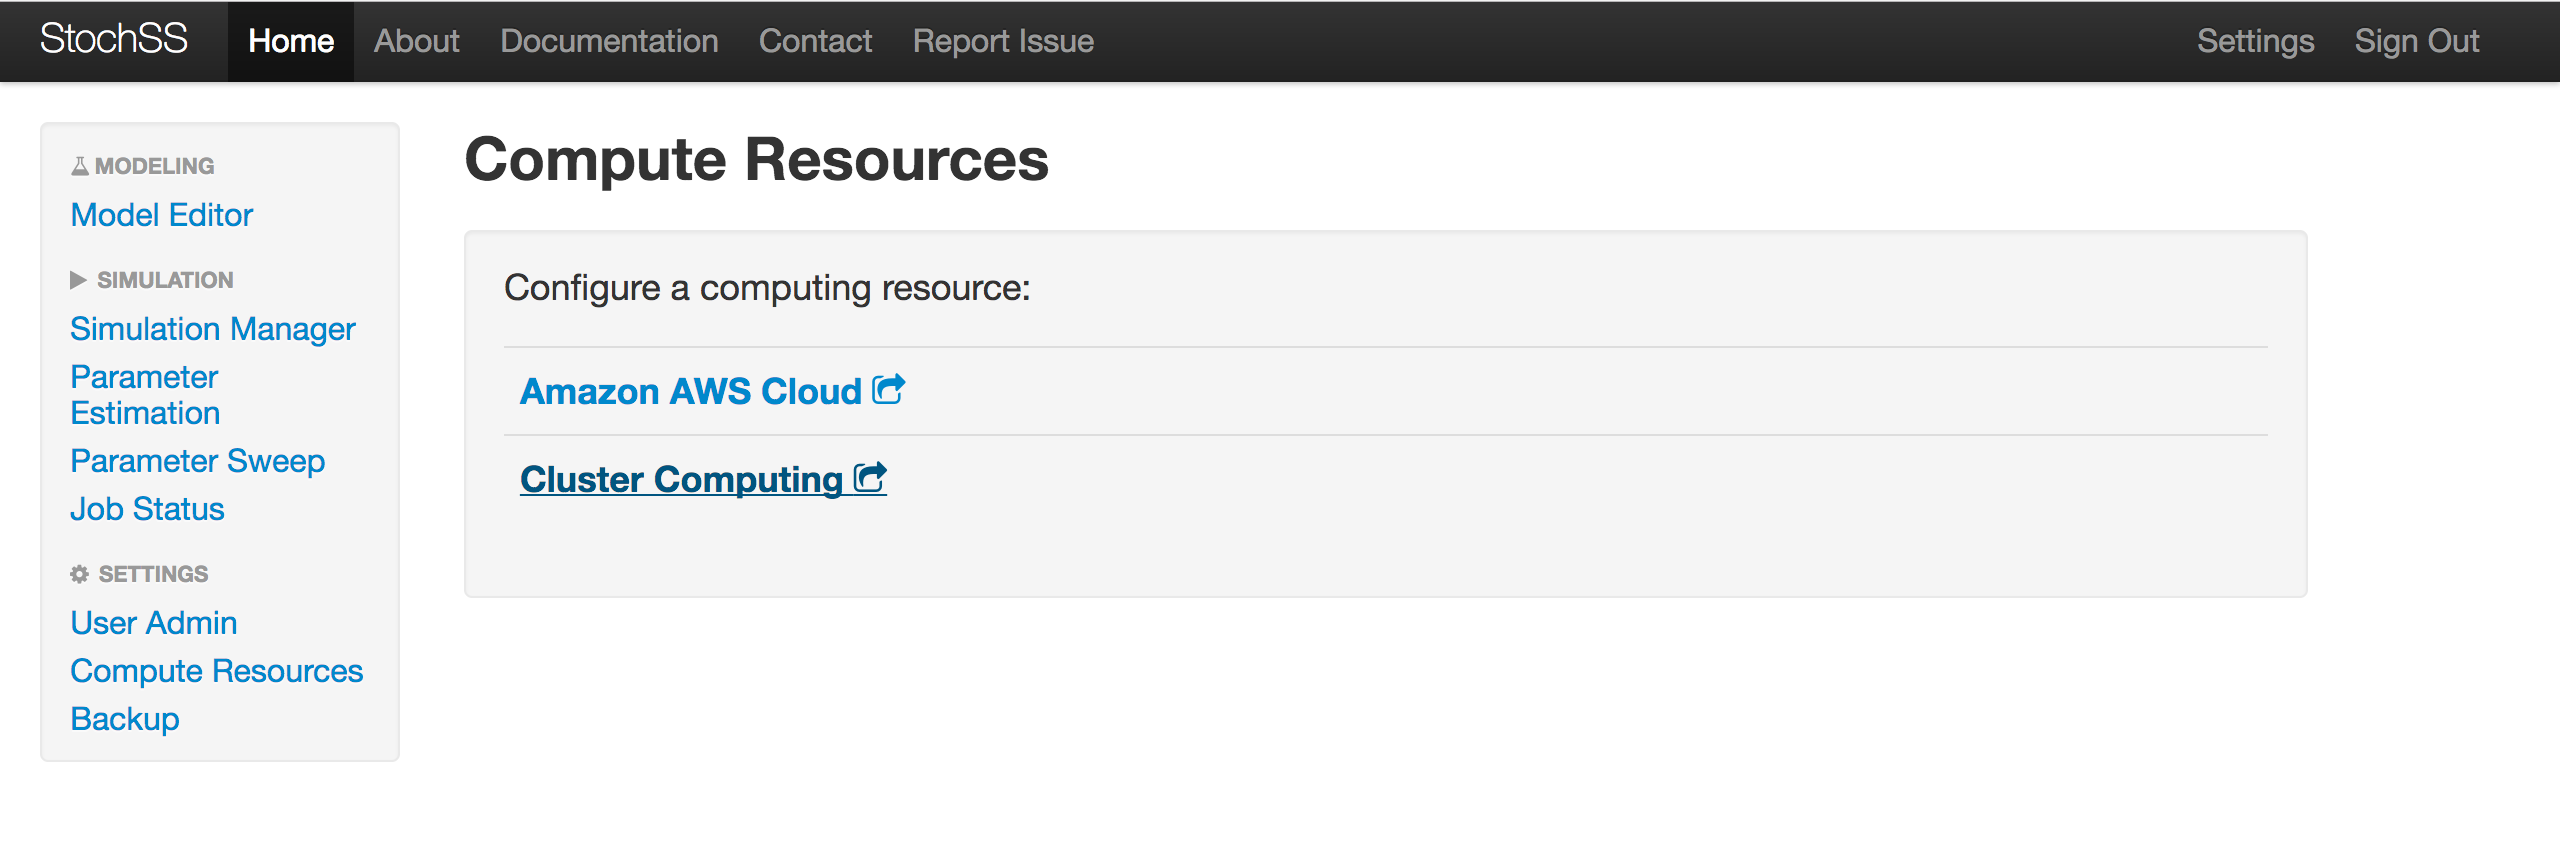
\includegraphics[width=100mm,scale=0.5]{cluster/figure1.png}
\caption{Compute Resources Page}
\label{fig:1}
\end{figure}

\begin{figure}[!ht]
\centering
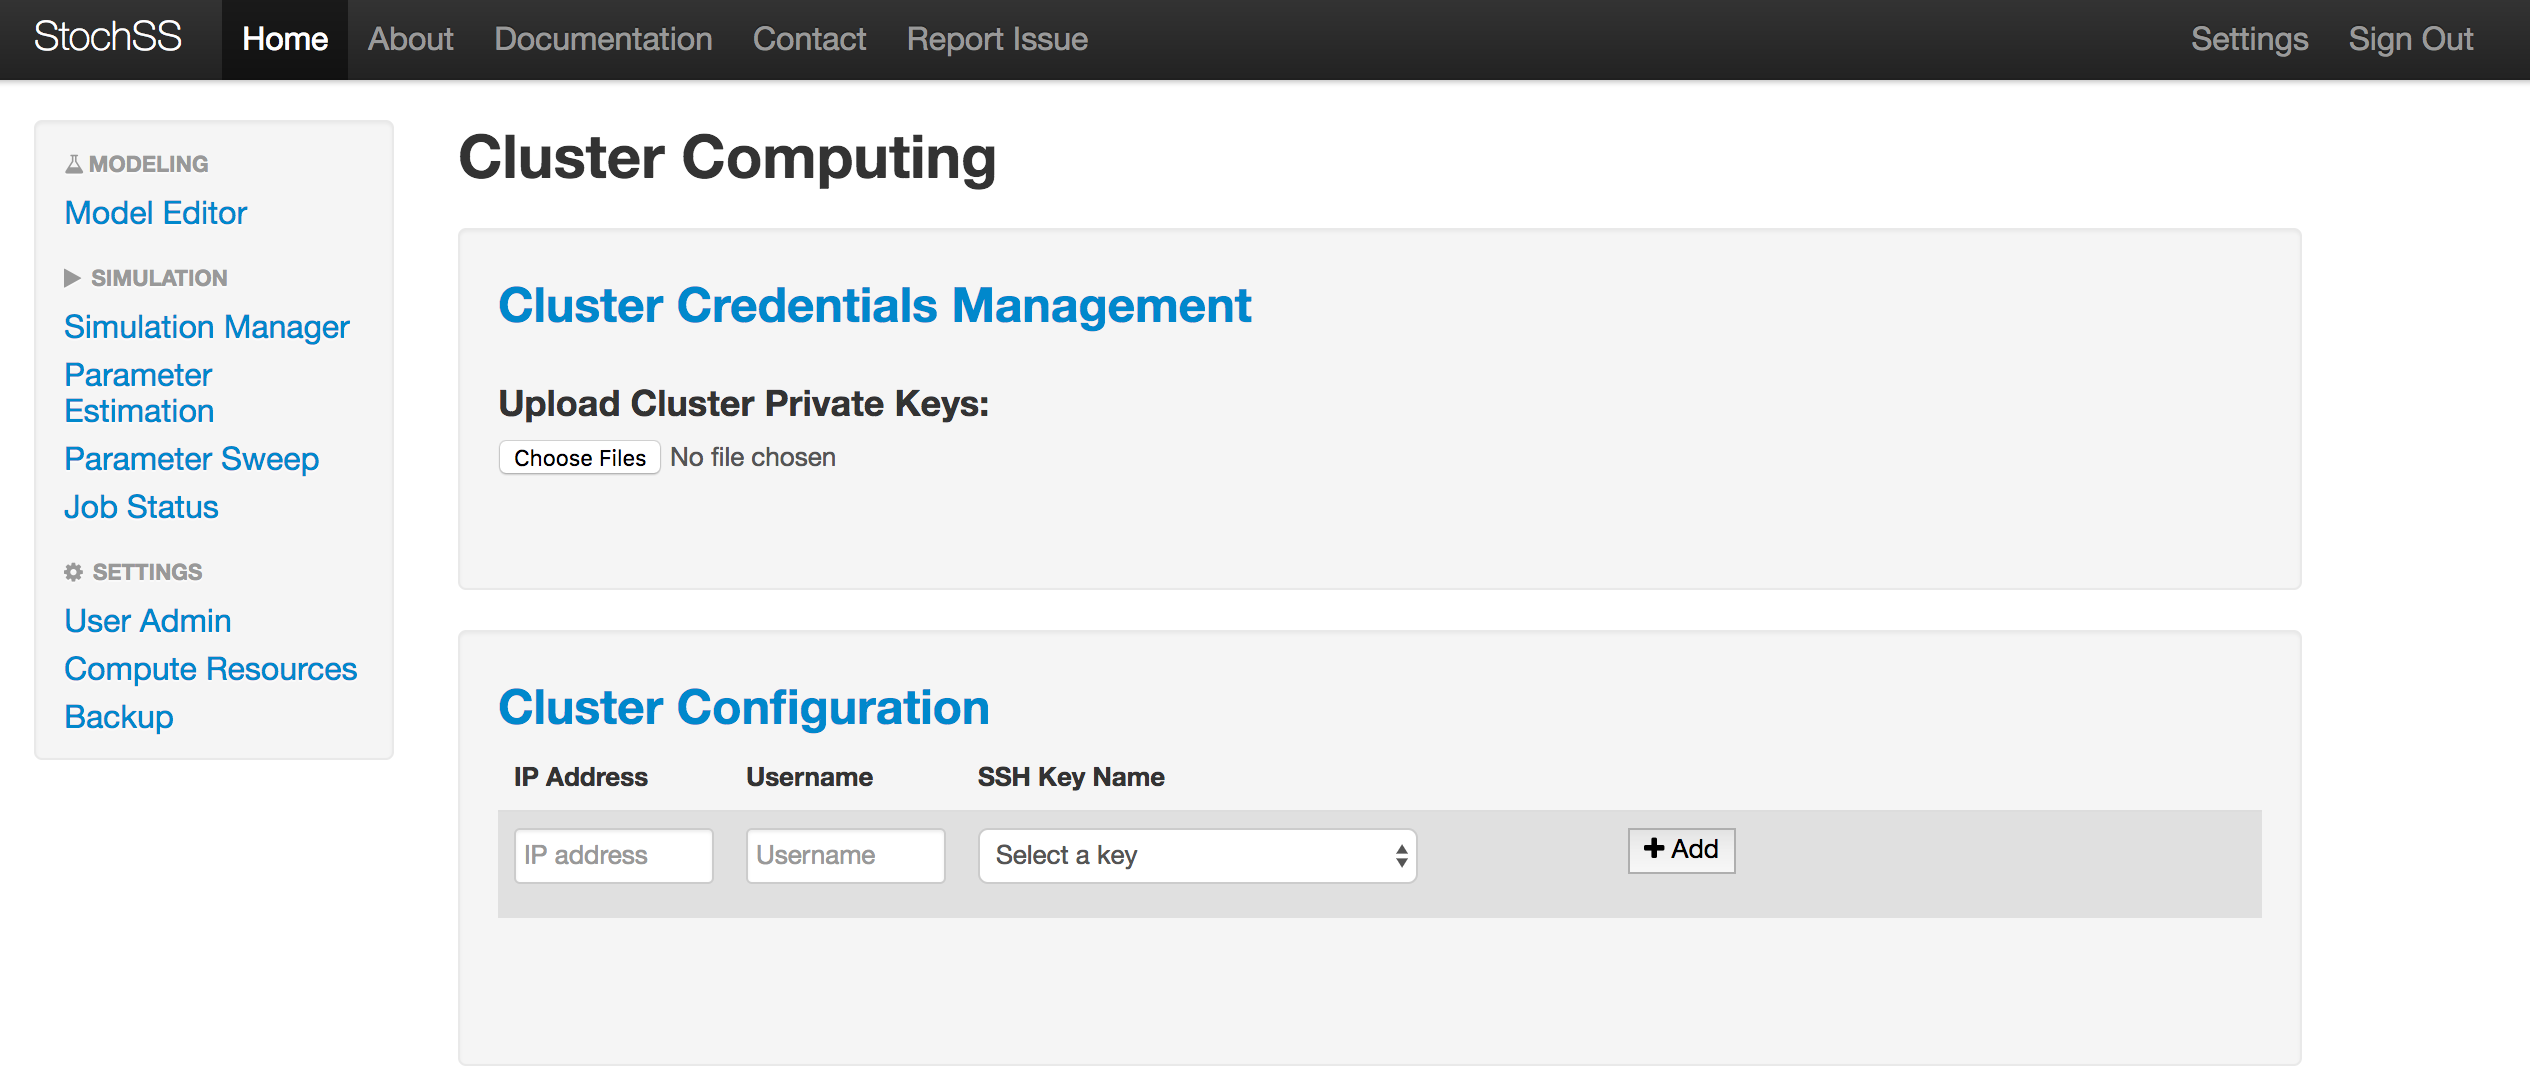
\includegraphics[width=100mm,scale=0.5]{cluster/figure2.png}
\caption{Configure Cluster Credentials}
\label{fig:2}
\end{figure}

\begin{enumerate}
\item Navigate to the main \textbf{Compute Resources} page. (Figure \ref{fig:1})
\item Click on \textbf{Cluster Computing}.
\item On the \textbf{Configure Cluster Credentials} page (Figure \ref{fig:2}):
  \begin{enumerate}
      \item Under \textit{Cluster Credentials Management}, click on \textbf{Choose Files} and upload your SSH key to the cluster.
      \item Under \textit{Cluster Configurations}, enter your username associated with the previously uploaded SSH key and the ip address of the cluster submit node. Click \textbf{Add}.
  \end{enumerate}
\end{enumerate}

\section{Running a job on a cluster}
After setting your credentials in StochSS, it is possible to use a cluster for the following types of experiments:
\begin{enumerate}
\item Parameter Sweeps
\item Simulations
\end{enumerate}

\subsection{An Example of performing an experiment on a cluster}
The following steps illustrate running a parameter sweep on a cluster. It is assumed that cluster credentials have been uploaded to StochSS, as described in section \ref{credentials}.
\begin{enumerate}
\item From the menu displayed in the left hand column of the screen, click on \textit {Parameter Sweep}.

\begin{figure}[!ht]
\centering
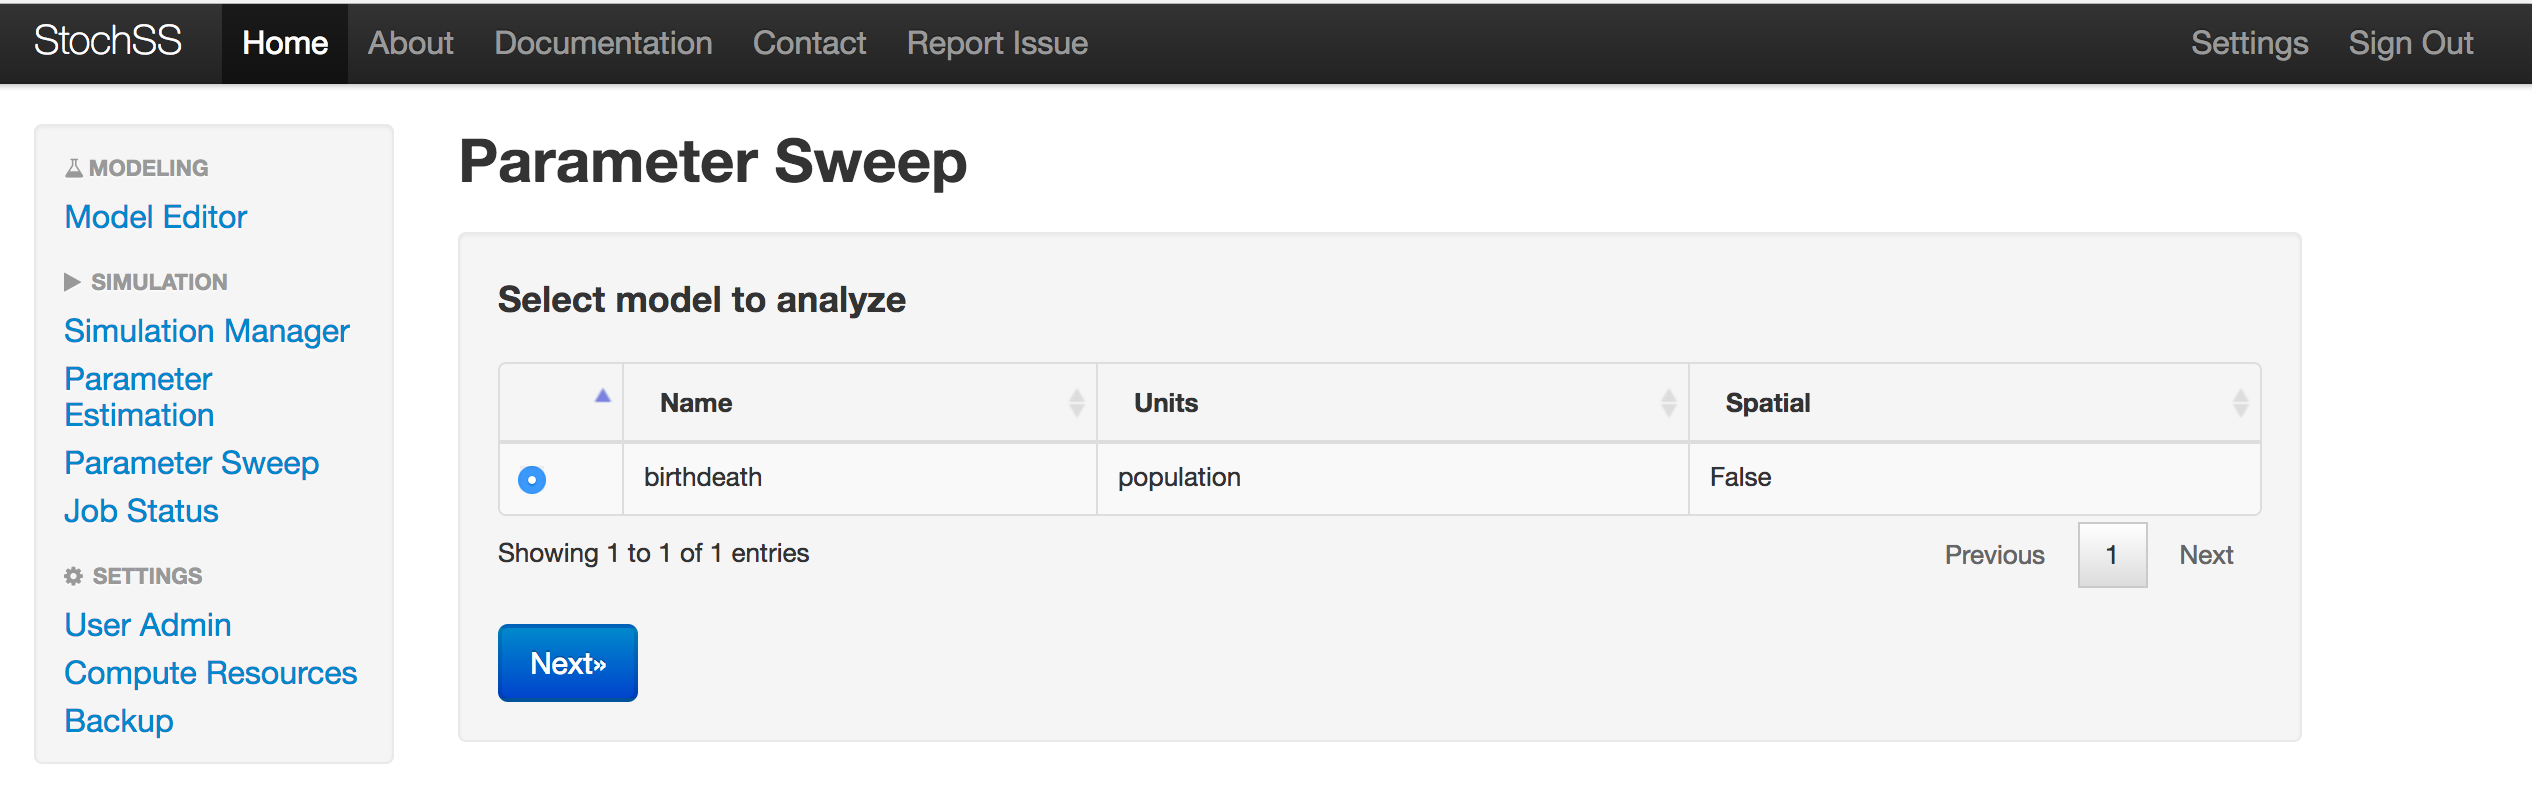
\includegraphics[width=100mm,scale=0.5]{cluster/figure3.png}
\caption{Select the model you wish to use and click next}
\label{fig:3}
\end{figure}

\begin{figure}[!ht]
\centering
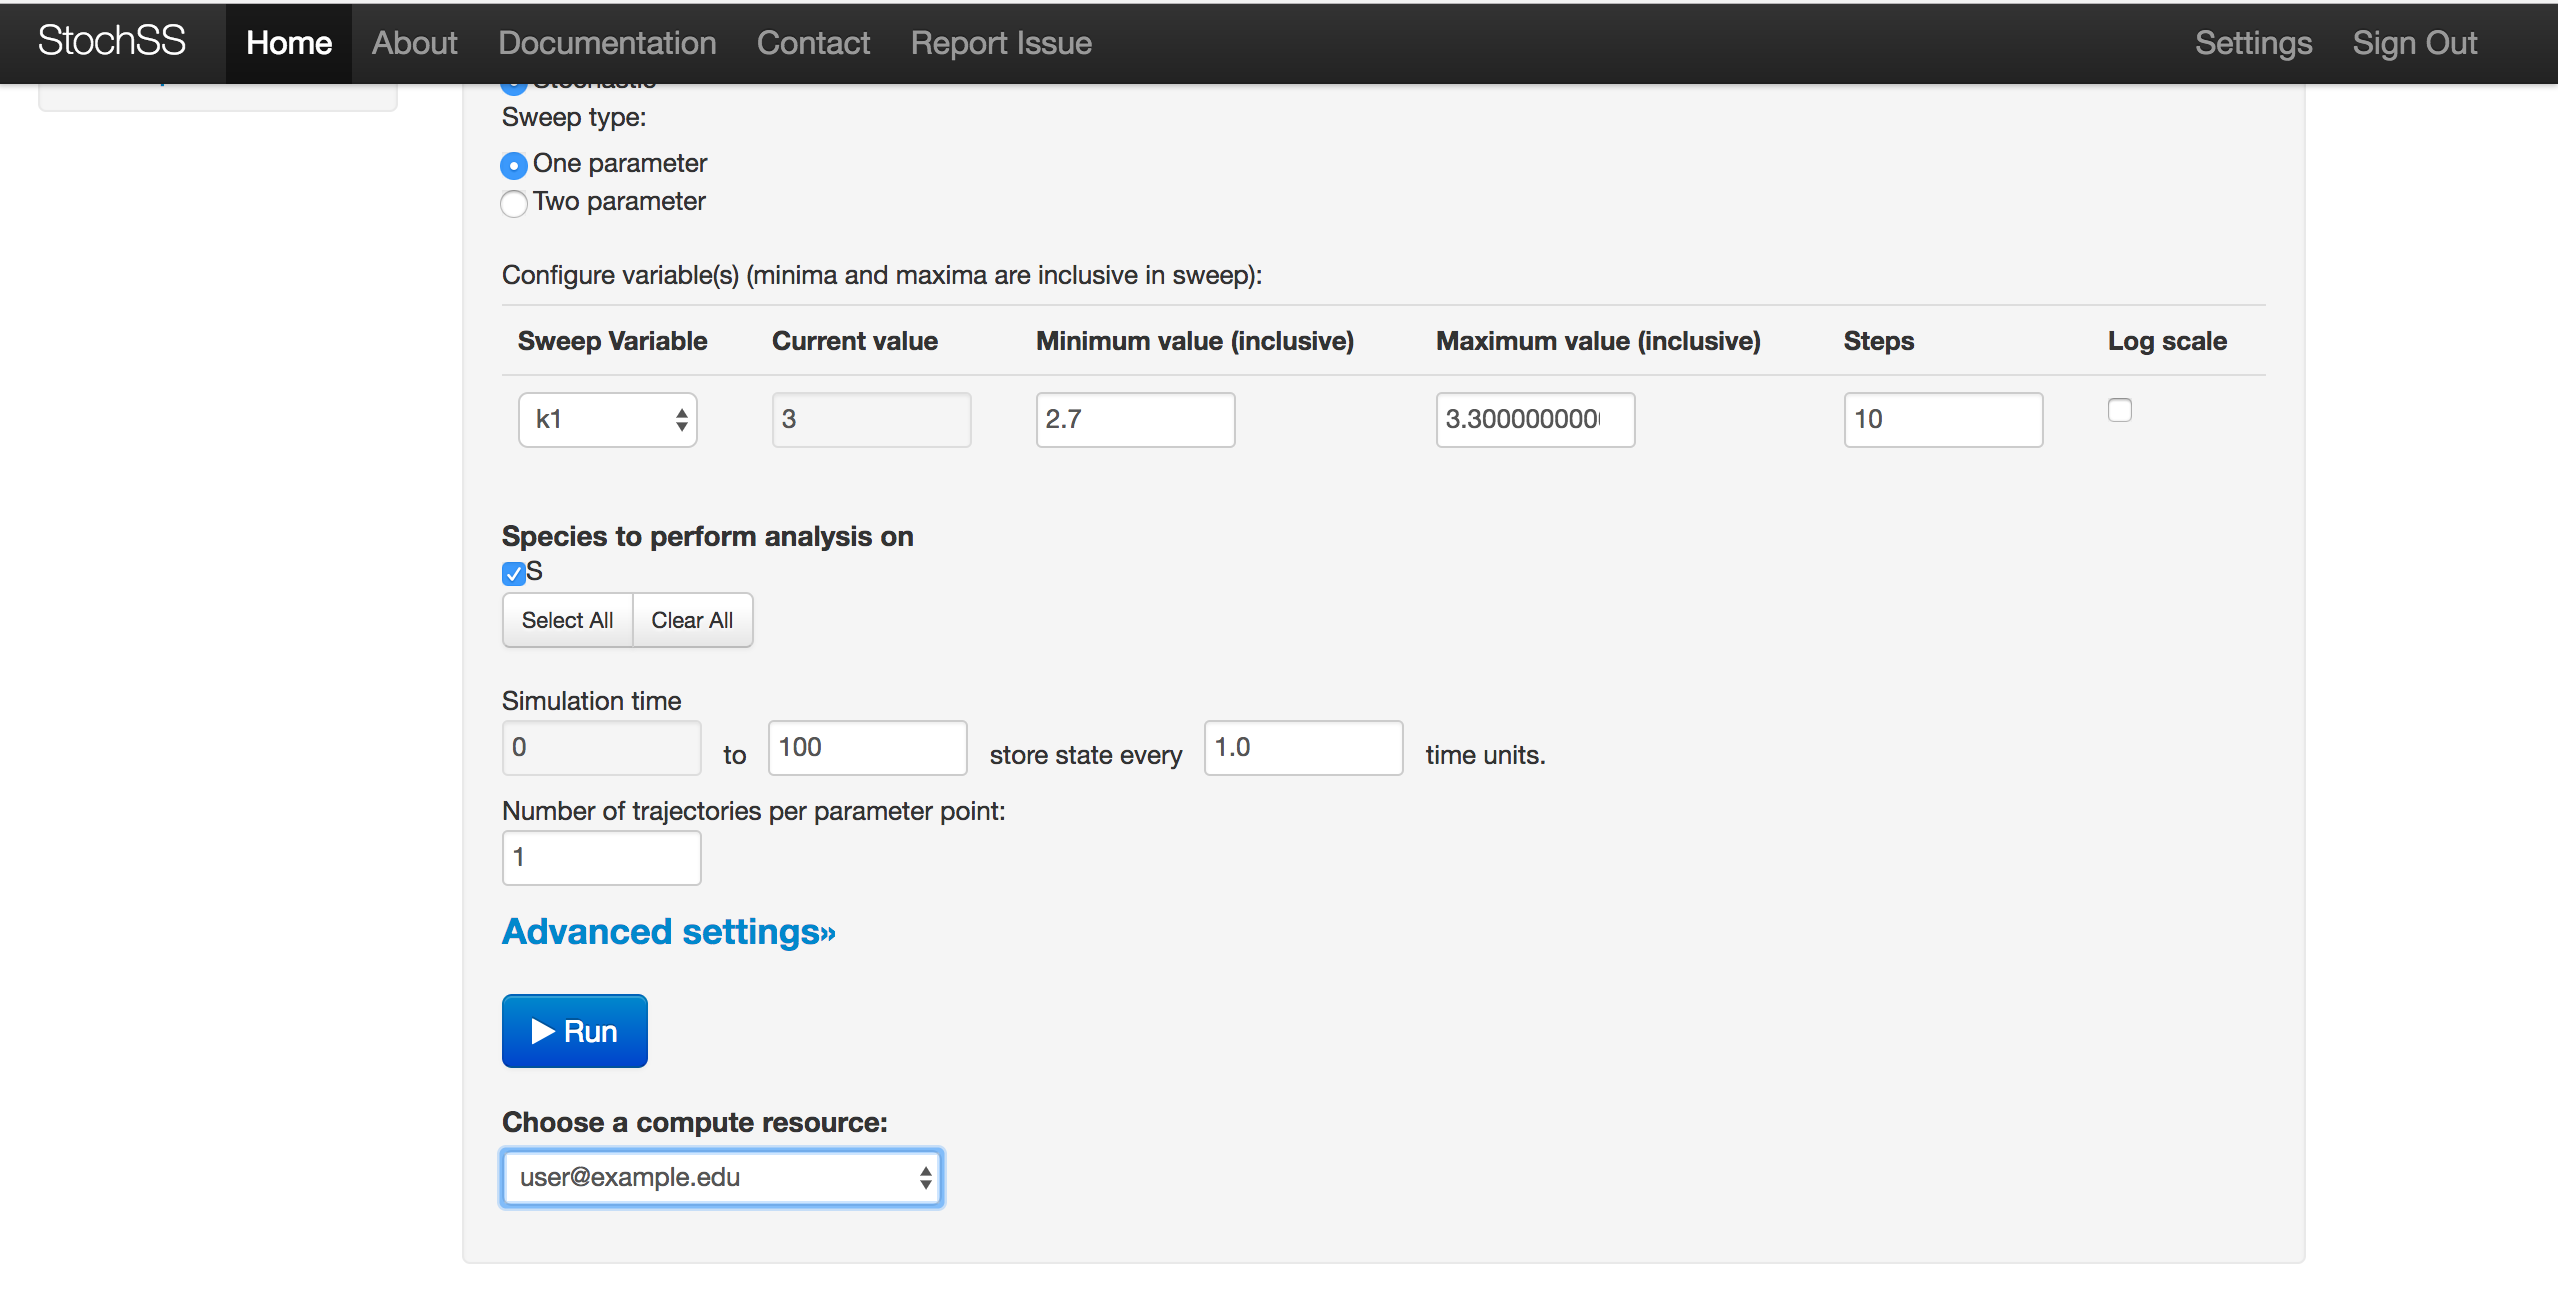
\includegraphics[width=100mm,scale=0.5]{cluster/figure4.png}
\caption{Select the cluster you wish to use}
\label{fig:4}
\end{figure}

\item Select the model you wish to use and click next. (Figure \ref{fig:3})
\item On the \textit{Run Parameter Sweep} page, configure different parameters of the experiment, if required and then at the bottom of the page, under \textit {Choose a compute resource}, click the drop-down menu and select the cluster you previously configured in StochSS. (Figure \ref{fig:4})
\item Click run to start the experiment on the cluster.
\item You will be automatically redirected to the results page when they are available.
\end{enumerate}
\end{document}
